\documentclass[conference]{IEEEtran}
\IEEEoverridecommandlockouts
\usepackage{cite}
\usepackage{amsmath}
\usepackage{graphicx}
\usepackage{booktabs}
\usepackage{xcolor}
\usepackage{url}
\usepackage[hidelinks]{hyperref}
\graphicspath{{figs/}}
% Items still to be filled from runs in progress are marked like this:
\newcommand{\TBD}[1]{\textcolor{red}{[TO UPDATE: #1]}}

\begin{document}

\title{Simulation-Based Evaluation of the Navigation Stack of ARC,\\an Adaptive Retail Companion for Shopping Carts}

\author{
\IEEEauthorblockN{Akshada Raghuvanshi}
\IEEEauthorblockA{School of Mechanical Engineering\\Vellore Institute of Technology, Chennai, India\\
\TBD{e-mail}}
\and
\IEEEauthorblockN{Manav Harish Kriplani}
\IEEEauthorblockA{School of Mechanical Engineering\\Vellore Institute of Technology, Chennai, India\\
\TBD{e-mail}}
\and
\IEEEauthorblockN{Dr. T. Christo Michael (guide)}
\IEEEauthorblockA{School of Mechanical Engineering\\Vellore Institute of Technology, Chennai, India\\
\TBD{e-mail}}
}

\maketitle

\begin{abstract}
ARC retrofits a supermarket cart into an assistive robot for elderly and mobility-impaired shoppers. We evaluate its ROS~2 navigation stack (RTAB-Map with lidar ICP odometry, a Dijkstra planner, a TEB-like controller and a behaviour tree) in a Gazebo store model under a baseline-first protocol. The median localisation error was 2--3~cm. The original stack completed 29 of 30 shopping missions without collision but needed 97 recoveries; all 62 controller aborts were Nav2's default progress timeout. The TEB-like controller reached 19 of 20 goals, against 13 for stock Regulated Pure Pursuit. Ordering the list by path cost cut driving time by 25--41\% but did not raise completion, because its short legs trip the same timeout. Unmapped boxes defeated the stack on 15 of 18 legs, and wheel-only odometry lost localisation twice. Relaxing the progress check to 0.25~m in 20~s and adding exact ordering completed all 30 lists in 26\% less time and 38\% less distance than the original stack ($p<10^{-6}$). On a bench, the stack drove the cart's motors from person detection on a Raspberry Pi~5. The wheels stopped within one 1~s telemetry period of every switch to WAIT, and a goal-reached race in the mission layer skipped two of four goals.
\end{abstract}

\begin{IEEEkeywords}
assistive robotics, autonomous shopping cart, ROS~2, Nav2, RTAB-Map, local planning, route ordering, simulation evaluation
\end{IEEEkeywords}

\section{Introduction}
Shopping is a routine task that elderly and mobility-impaired people often find tiring: pushing a loaded cart, walking between distant shelves and backtracking through aisles \cite{estember2017}. Service robots that anticipate the needs of elderly users are an active research area \cite{yueh2026}. ARC (Adaptive Retail Companion) is a modular retrofit kit that turns a conventional supermarket cart into an assistive platform. The cart leads the user to the items on a shopping list, follows them, or waits.

This paper does not propose a new algorithm. It reports a systematic, reproducible evaluation of ARC's integrated navigation software before hardware deployment. We ask four questions: how accurate localisation is (A1); how reliably the stack completes shopping missions (A2, B1); whether its optimising local controller is justified over a standard one (A3); and how it handles obstacles that are not on its map (A4). We also ask whether the order in which items are visited matters, offline (C1) and when driven (C2).

Related work (Section~\ref{sec:rw}) shows that neither the retrofit idea nor shopping-list ordering is new, so this paper claims measured evidence, not a first. The contributions are: (i) a baseline-first test protocol with automatic integrity checks, in which variants are run on the same tasks and seeds as the original; (ii) measured performance of the original stack on seven tests; (iii) five integration-level findings traced to specific code and configuration; (iv) a paired test of two candidate fixes on the original tasks, leading to a recommendation; and (v) a bench hardware-in-the-loop test with the real drive motors and on-board person detection.

\section{Related Work}
\label{sec:rw}
\textit{Shopping robots.} RoboCart guided visually impaired shoppers through a grocery store \cite{kulyukin2005}, and later carts added ROS-based deep-learning perception \cite{su2016} and customer-oriented services \cite{chiang2016}. Dedicated platforms carry the strongest field evidence: CompaRob assisted elderly users in real grocery stores \cite{sales2016}, and Yao et al.\ tracked shoppers under shelf occlusion in a real supermarket \cite{yao2026}. Retrofit systems are older. Nishimura et al.\ attached a detachable drive and stereo sensor module to an ordinary cart for person following \cite{nishimura2007}. Kohtsuka et al.\ attached a driving unit and onboard computer to a conventional cart, with laser-based following \cite{kohtsuka2011}. Neither reports map-based navigation of a shopping list. Retrofit autonomy is better established on wheelchairs, for example the modular RTAB-Map-based shared-control system of Ramaraj et al.\ \cite{ramaraj2024} and detachable propulsion units for manual wheelchairs \cite{kang2026}.

\textit{Person following and perception.} Person-following robots have used stereo detection \cite{satake2009}, RGB-D tracking \cite{luber2011,basso2012}, and learned detectors with fuzzy or vision-based control \cite{aye2019,yong2022}. ARC's bench test uses a YOLOv8 detector \cite{yaseen2024} with ByteTrack association \cite{zhang2022}.

\textit{Shopping-list ordering.} Visiting a list of items is a sequencing problem related to warehouse order picking. Picking has exact solutions for parallel-aisle layouts \cite{ratliff1983} and a large heuristic literature \cite{dekoster2007}. Nearest-neighbour ordering is not optimal in the worst case \cite{rosenkrantz1977}; local search such as 2-opt improves a tour without guaranteeing the optimum \cite{croes1958}, and the Held--Karp dynamic program is exact and practical for short lists \cite{held1962}. Closest to this work, Choi et al.\ compute Dijkstra distances between list items in a supermarket model and order the items with a genetic algorithm. Their study is simulation-only, with a potential-field local planner outside ROS \cite{choi2025}. Within the scope of our search, we are not aware of a study that measures, inside a ROS~2 navigation stack, how far simple ordering rules fall from the optimum and whether the planned savings survive execution by the local controller; C1 and C2 address this.

\textit{Planning and control.} ARC uses standard methods: Dijkstra search \cite{dijkstra1959}, the Nav2 framework \cite{macenski2020} and timed-elastic-band control \cite{rosmann2012,rosmann2017}. Common alternatives for local control are the dynamic window approach \cite{fox1997} and its fuzzy variants \cite{rachman2025}; TEB itself has been extended for cluttered environments \cite{wu2021}. Li et al.\ fuse Dijkstra with an improved TEB and report a smaller turning radius and shorter operation time \cite{li2025}. ARC's planner and controller are therefore engineering components, not algorithmic contributions. For localisation, alternatives include feature-based visual SLAM \cite{murartal2017,tourani2022}, lidar-inertial odometry \cite{shan2020} and multi-sensor 2D mapping \cite{altawil2025}.

\section{System Overview}
Fig.~\ref{fig:arch} shows the navigation pipeline. A 2D lidar feeds ICP scan-matching odometry (libpointmatcher \cite{pomerleau2013}). RTAB-Map \cite{labbe2019} builds a map and, once the map is locked, localises against it. A Dijkstra planner computes the global path on the occupancy grid. The path hand-over node passes the path to Nav2's controller server, which runs ARC's TEB-like controller. A motion gate scales the controller's command according to the behaviour-tree \cite{colledanchise2018,iovino2022,ogren2022} mode (FOLLOW, WAIT, LEAD or emergency stop). The shopping manager sends one goal per item and waits for a ``goal reached'' message before prompting the user to continue. The software runs on ROS~2 \cite{macenski2022}.

\begin{figure*}[t]
\centering
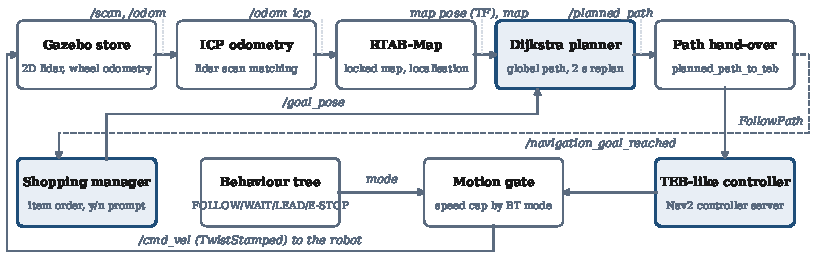
\includegraphics[width=\textwidth]{fig1_architecture}
\caption{ARC navigation pipeline as tested. Shaded boxes are ARC's own planning, control and mission components. The dashed line is the ``goal reached'' message that advances the shopping list.}
\label{fig:arch}
\end{figure*}

\section{Experimental Method}

\subsection{Setup}
All tests ran in Gazebo \cite{koenig2004} on one laptop (Table~\ref{tab:setup}). The robot model is a stand-in, because the cart hardware was not yet integrated. ARC's source files and parameters were not modified, with one exception made before testing: the controller's maximum turn rate was lowered from 1.0 to 0.5~rad/s, after a fast turn caused an ICP jump in a pilot run. All ROS and Gazebo traffic was restricted to the local machine, after two runs failed when the Wi-Fi connection changed.

\begin{table}[t]
\caption{Test Configuration}
\label{tab:setup}
\centering
\footnotesize
\begin{tabular}{@{}p{2.0cm}p{5.9cm}@{}}
\toprule
Component & Configuration \\
\midrule
Software & Ubuntu 24.04, ROS 2 Jazzy, Gazebo Harmonic \\
Robot model & TurtleBot3 Burger: differential drive, 2D lidar, wheel odometry \\
Environment & Compact store: three gondola units, checkout, tea shelf, fridge, produce; 29 item locations in 9 driving stops \\
Map & 0.05~m grid, about $180\times160$ cells, rebuilt each session \\
Localisation & RTAB-Map in localisation mode, ICP odometry \\
Global planner & Dijkstra, 8-connected, 0.20~m inflation, unknown cells cost $5\times$, replans every 2~s \\
Local controller & TEB-like (Nav2): $v_{\max}=0.15$~m/s, $\omega_{\max}=0.5$~rad/s, $\dot\omega_{\max}=1.0$~rad/s$^2$ \\
Behaviour & LEAD mode; motion gate caps speed at 0.10~m/s \\
\bottomrule
\end{tabular}
\end{table}

\textbf{Map acceptance.} Each session began with an automated 11-waypoint mapping drive. A map was locked only if the map pose matched Gazebo's true pose within 0.05~m at the start area. Up to three loop-closing passes were allowed to reach this. After locking, the map also had to match within 0.15~m and $5^\circ$; otherwise it was rebuilt.

\subsection{Tests and Protocol}
Table~\ref{tab:tests} lists the tests. The study is baseline-first. In phase~1 the original ARC is measured unchanged. In phase~2, variants run on the same tasks and seeds, from copies of the configuration, so ARC's files stay untouched. In phase~3 the variants are compared with the baseline on identical tasks. A separate test kit sends goals to the planner exactly as the shopping manager does, and logs all data.

\begin{table}[t]
\caption{Tests (Phase 1 Unless Noted)}
\label{tab:tests}
\centering
\footnotesize
\begin{tabular}{@{}lp{4.6cm}l@{}}
\toprule
Test & Task & Trials (seed) \\
\midrule
A1 & Localisation error, logged in all tests & all samples \\
A2 & Random lists of 3--12 items, typed order & 30 (7) \\
A3 & Start--goal pairs, TEB-like vs.\ RPP \cite{macenski2023} & 20 each (5) \\
A4 & Pairs $\geq$2.5~m apart; 1--3 boxes placed on the path after planning & 20 (9) \\
B1 & First 10 A2 lists, wheel odometry only & 10 (7) \\
C1 & Route length by ordering method, offline & 50 per size \\
C2 & Lists driven in typed, nearest-next and exact order & 30 $\times$ 3 (21) \\
A2-pc & A2 with a relaxed progress check (phase 2) & 30 (7) \\
A2-final & A2-pc with exact ordering (phase 2) & 30 (7) \\
\bottomrule
\end{tabular}
\end{table}

\subsection{Metrics}
\textit{Localisation error:} the distance between the map pose and Gazebo's true pose, sampled every 2~s. The true pose is time-stamped at the midpoint of its request, and the map pose is looked up at that time. A loss episode is an excursion above 0.5~m or $15^\circ$.

\textit{Leg success:} a leg is a drive to one stop. It succeeds when ARC reports ``goal reached'' with the robot within 1.0~m of the goal, which is the planner's goal-snapping radius. A mission succeeds when all its legs do.

\textit{Recoveries:} controller aborts plus goal re-sends. The kit re-sends a goal once after an abort or a 40~s stall.

\textit{Contact (A4):} the clearance between the robot's edge and a box, computed from true positions with a 0.105~m robot radius. A clearance of 0 or less counts as contact.

\textit{Route cost (C1, C2):} the Dijkstra path length on a grid built from the same map. This grid uses a 0.15~m radius and blocks unknown cells, so it approximates the planner's costs rather than reproducing them. The exact order is the Held--Karp optimum.

A run stops automatically if the map pose stays more than 1.0~m from the truth for 10~s, or if simulation time freezes for 15~s; the rows logged so far are kept. Paired differences use the Wilcoxon signed-rank test \cite{wilcoxon1945}. Binary outcomes use the sign test on discordant pairs.

\subsection{Measurement Integrity}
Several faults in the test chain itself were found and corrected during the campaign. Gazebo acknowledged the removal of test boxes that remained in the world; the affected A4 run was voided and kept as evidence, and every removal is now verified against Gazebo's model list. A stale replan of the previous goal was once taken as the next leg's path, so paths and arrivals now count only if they end within 1.0~m of the current goal. An automatic re-check of all earlier legs found one false arrival in A3 (RPP), which is counted as a failure. Gazebo's pose service was silent for 15~s or more 418 times during C2, so driven distances from C2 are not reported. Every exclusion is recorded in a timestamped lab notebook.

\section{Results}

\subsection{Localisation Accuracy (A1)}
With ICP odometry, the median error was 0.018--0.038~m in every configuration (Fig.~\ref{fig:loc}). Between 91.2\% and 97.9\% of samples fell within the 0.15~m and $5^\circ$ band. Excursions from the band were mostly in heading: the band is tight on yaw, and the median heading error was 0.5--1.0$^\circ$. All large errors after the pilot run came from two distinct events, not from gradual degradation. Lidar odometry failed after contact: with boxes in A4 (Section~\ref{sec:a4}) and once with a shelf in A2-pc (Section~\ref{sec:p2}). Early maps were offset by about 0.25~m when the final leg home had not been loop-closed; the pre-lock start-area check removed this.

\begin{figure}[t]
\centering
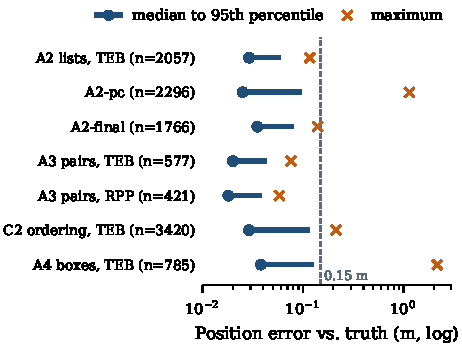
\includegraphics[width=\columnwidth]{fig2_localisation}
\caption{Localisation error per configuration with ICP odometry (samples every 2~s). The A4 and A2-pc maxima come from lidar-odometry failures after contact with a box and a shelf.}
\label{fig:loc}
\end{figure}

\subsection{Mission Reliability (A2)}
The original stack completed 29 of 30 missions and reached 143 of 144 stops with no contact. Only 96 stops (67\%) were reached at the first attempt, and the runs needed 97 recoveries in total. All 62 controller aborts were Nav2 code 105 (``failed to make progress''). ARC's configuration defines no progress checker, so Nav2 uses its default: the robot must move 0.5~m within 10~s. At 0.10--0.15~m/s, and slower while turning into an aisle, legitimate manoeuvres can fail this check. The path hand-over has no recovery, so without the kit's single re-send each abort would leave the shopping manager waiting indefinitely. The phase-2 variant A2-pc relaxes the check to 0.25~m within 20~s (Section~\ref{sec:p2}).

\subsection{Local Controller Comparison (A3)}
Table~\ref{tab:a3} compares the controllers on the same 20 pairs, with Pure Pursuit limited to the TEB-like controller's speed, turn rate and angular acceleration. Pure Pursuit mostly failed by refusing to move. Its collision check found no admissible command in aisles narrowed by the 0.20~m inflation (code 106). The TEB-like controller was more reliable but less smooth. Its mean absolute angular acceleration was 0.220~rad/s$^2$ against 0.083 for Pure Pursuit (Wilcoxon, $n=19$, $p=2.7\times10^{-5}$), and it reversed steering 1.88 times per metre against 0.80. Pure Pursuit used stock collision and look-ahead settings. The result therefore shows that stock Pure Pursuit is unsuited to these aisles, not that a tuned version could not work. On the 12 pairs both controllers completed, mission time (68.2~s against 62.8~s) and driven distance (4.73~m against 4.29~m) did not differ significantly (Wilcoxon, $p=0.23$ and $p=0.38$).

\begin{table}[t]
\caption{Controller Comparison on 20 Identical Pairs (A3)}
\label{tab:a3}
\centering
\footnotesize
\begin{tabular}{@{}lcc@{}}
\toprule
Measure & TEB-like & RPP (stock) \\
\midrule
Goals reached & 19/20 & 13/20 \\
Reached at first attempt & 12/20 & 10/20 \\
Recoveries & 17 & 24 \\
Dominant abort & 105 (no progress) & 106 (no valid control) \\
Mean $|\dot\omega|$ (rad/s$^2$) & 0.220 & 0.083 \\
Steering reversals per m & 1.88 & 0.80 \\
Median localisation error (m) & 0.020 & 0.018 \\
\bottomrule
\end{tabular}
\end{table}

\subsection{Unmapped Obstacles (A4)}
\label{sec:a4}
Boxes measuring $0.20\times0.20\times0.35$~m were placed on the planned path after planning. They went at 45\%, then 70\%, then 30\% of the path length, offset 0.15~m to alternating sides, and never within 0.6~m of the start or goal. Over all 20 pairs, 18 were driven with boxes and two without, as logged by the runner; both box-free pairs reached their goals. The stack reached 3 of the 18 goals with boxes and touched a box in 17 (Table~\ref{tab:a4}). The median minimum clearance was $-0.027$~m (worst $-0.061$~m), and 14 of the 15 failures were controller aborts. The outcome follows from the architecture. The global planner uses the locked map, so it never sees the boxes. The hand-over node ignores new paths while one is being followed. Avoidance is therefore left to the local controller alone, which can bend around one box but not pass two or three. In two of the 3-box legs, ICP odometry failed shortly after contact and never recovered. Its log shows every later match rejected for exceeding the 0.2~m correction limit. The likely cause is wheel slip against the box, which would corrupt ICP's initial guess; this is consistent with the logs but was not measured directly.

\begin{table}[t]
\caption{Outcome by Number of Boxes on the Path (A4, All 20 Pairs)}
\label{tab:a4}
\centering
\footnotesize
\begin{tabular}{@{}cccc@{}}
\toprule
Boxes & Legs & Goal reached & Contact \\
\midrule
1 & 7 & 3 & 6 \\
2 & 4 & 0 & 4 \\
3 & 7 & 0 & 7 \\
\midrule
All & 18 & 3 & 17 \\
\bottomrule
\end{tabular}
\end{table}

\subsection{Shopping-List Ordering (C1, C2)}
Offline, typed order produced routes 23\% to 94\% longer than the optimum for 3 to 12 items (Fig.~\ref{fig:c1}). Nearest-next on path cost stayed within 1--7\%, better than nearest-next on straight-line distance (3--9\%), because shelves block the direct line. The exact solution took at most 4.8~ms for 12 items, so the optimum is affordable on board.

\begin{figure}[t]
\centering
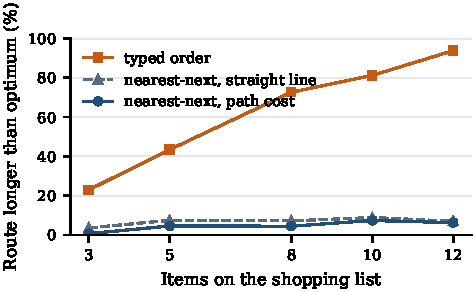
\includegraphics[width=\columnwidth]{fig3_c1_ordering}
\caption{Offline route length relative to the exact optimum (C1, 50 random lists per size). Route cost is Dijkstra path length on the test grid.}
\label{fig:c1}
\end{figure}

Driven, the exact order was faster than typed order on 30 of 30 lists (one-sided sign test, $p\approx9\times10^{-10}$; Fig.~\ref{fig:c2}). Median route length fell by 32\%, 42\% and 51\%, and median time by 25\%, 34\% and 41\%, for 5, 8 and 12 items. On the 12 lists that both strategies completed, the time saved was still 30\% (range 14--43\%). The saving is therefore not an artefact of failed legs ending early.

Completion did not improve: 19 of 30 missions with typed order, 15 with exact and 13 with nearest-next ordering. The difference between exact and typed order is not significant (7 against 3 discordant lists, $p=0.34$). Ordered routes consist mostly of short hops between neighbouring shelves: 90\% of legs were under 3.5~m, against 44\% with typed order. Legs of 2--3.5~m, which often begin with a turn into an aisle, failed most often (18\%). First-attempt arrivals fell from 93 of 181 to 72 (exact) and 63 (nearest-next). Ordering thus exposes the same progress-check aborts as A2. With the relaxed check, exact ordering completed all 30 A2 lists (Section~\ref{sec:p2}).

\begin{figure}[t]
\centering
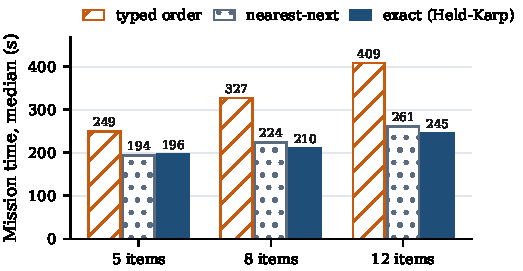
\includegraphics[width=\columnwidth]{fig4_c2_time}
\caption{Median mission time by ordering strategy and list size (C2, 10 lists per size, all missions including those with failed legs).}
\label{fig:c2}
\end{figure}

\subsection{Wheel-Only Odometry (B1)}
Wheel odometry accumulates error without bound \cite{thrun2005}. With wheel odometry in place of ICP odometry, localisation was as accurate as before while it held (median 0.023~m). It was lost twice, after about 73~m and 48~m of driving; overall, 4 of 5 lists were completed and 22 of 23 stops reached. By a rule fixed in advance, B1 was stopped at the second loss. Fig.~\ref{fig:b1} shows the first loss. The wheel-odometry error was 1--2~m throughout. RTAB-Map's map-to-odometry correction absorbed it and kept the map error at a few centimetres, until the correction froze from about $t=1388$~s. From then on, the map error grew past the 1.0~m loss threshold within about 80~s. RTAB-Map had not crashed: it kept processing scans with its map intact. Its log shows localisations rejected as ``wrong loop closure'' because the optimised graph disagreed with the odometry beyond its error-ratio limit. A plausible mechanism, consistent with but not proven by these logs, is that large wheel drift makes correct matches look inconsistent, so they are rejected and the drift keeps growing.

\begin{figure}[t]
\centering
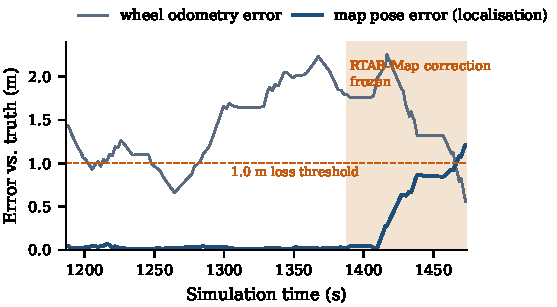
\includegraphics[width=\columnwidth]{fig5_b1_wheel}
\caption{First B1 localisation loss. The map pose stays accurate while RTAB-Map corrects the wheel drift, then diverges once its correction stops updating (shaded). Gaps are periods without a true-pose sample.}
\label{fig:b1}
\end{figure}

\subsection{Phase 2: Progress Check and Ordering (A2-pc, A2-final)}
\label{sec:p2}
Both variants drove the 30 A2 lists (seed 7) on the same stack, changing only a copy of the controller configuration. A2-pc relaxes the progress check to 0.25~m within 20~s. A2-final adds the exact (Held--Karp) visiting order. Table~\ref{tab:p2} and Fig.~\ref{fig:p2} summarise the three configurations, and Fig.~\ref{fig:p2pair} pairs them list by list.

\begin{table}[t]
\caption{Original Stack and Phase-2 Variants on the 30 A2 Lists}
\label{tab:p2}
\centering
\footnotesize
\setlength{\tabcolsep}{3.5pt}
\begin{tabular}{@{}lccc@{}}
\toprule
Measure & A2 & A2-pc & A2-final \\
\midrule
Progress check & 0.5~m/10~s & 0.25~m/20~s & 0.25~m/20~s \\
Visiting order & typed & typed & exact \\
Missions completed & 29/30 & 29/30 & 30/30 \\
Stops reached & 143/144 & 140/141 & 144/144 \\
Reached at first attempt & 96 (67\%) & 136 (96\%) & 133 (92\%) \\
Recoveries (aborts) & 97 (62) & 4 (0) & 13 (2) \\
Median mission time (s) & 255 & 259 & 218 \\
Mean driven distance (m) & 18.6 & 18.9 & 11.6 \\
Shelf contacts & 0 & 1 & 0 \\
Mean $|\dot\omega|$ (rad/s$^2$) & 0.211 & 0.231 & 0.273 \\
Steering reversals per m & 2.07 & 2.13 & 3.01 \\
Loc.\ error, med./max (m) & 0.029/0.117 & 0.025/1.149 & 0.035/0.140 \\
\bottomrule
\end{tabular}
\end{table}

\begin{figure*}[t]
\centering
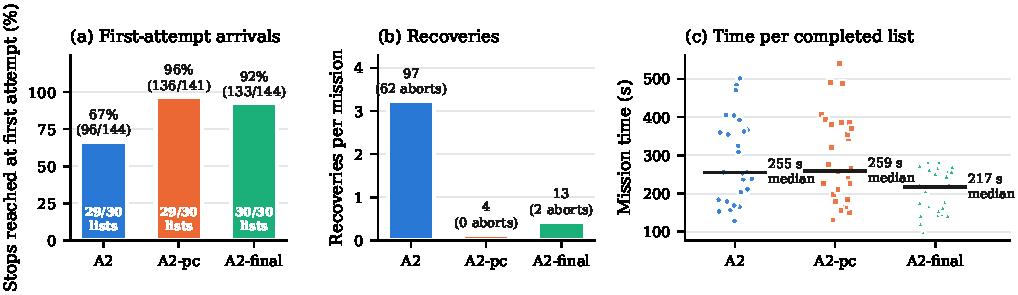
\includegraphics[width=\textwidth]{fig6_phase2}
\caption{Original stack (A2) and the phase-2 variants on the same 30 lists. (a) Stops reached without an abort or re-send, with completed lists inside the bars. (b) Recoveries per mission; labels give totals and the controller aborts among them. (c) Mission time of every completed list; the bar is the median.}
\label{fig:p2}
\end{figure*}

\textit{Progress check alone.} The relaxed check removed the aborts it was meant to remove. Controller aborts fell from 62 to 0, recoveries from 97 to 4, and stops reached at the first attempt rose from 67\% to 96\%. Completion did not change (29 of 30 lists each; one discordant list each way). It was not free. On the 28 lists both completed, missions took 3.8\% longer (287.5~s against 277.0~s, Wilcoxon $p=1.4\times10^{-4}$), and only 4 lists were faster (Fig.~\ref{fig:p2pair}). Driven distance did not differ significantly ($p=0.07$). In one leg the robot pressed against a shelf (clearance $-0.055$~m) while covering 1.0~m of a 7.1~m path in 42~s. Lidar odometry then failed and did not recover, as after box contact in A4, and the run stopped on the 1.0~m loss rule. A more lenient check lets a stuck robot keep pushing for up to 20~s instead of 10~s, which is a plausible link. One event in 141 legs cannot establish a rate, and A2 itself had no contact.

\textit{Progress check with exact ordering.} A2-final completed all 30 lists and all 144 stops with 13 recoveries and no contact. On the 29 lists both completed, it took 26\% less time than the original stack (207.4~s against 281.0~s, $p=5.1\times10^{-7}$) and drove 38\% less (11.5~m against 18.6~m, $p=1.2\times10^{-7}$). It was faster on 27 of the 29 lists, with a median per-list change of $-23\%$. Against A2-pc, which differs only in the visiting order, the savings were 28\% in time and 39\% in distance ($p=7.1\times10^{-8}$ and $7.5\times10^{-9}$). The cost is smoothness: shorter routes contain more turns per metre, so mean $|\dot\omega|$ rose from 0.211 to 0.273~rad/s$^2$ ($p=8.1\times10^{-4}$) and steering reversals from 2.1 to 3.0 per metre.

\begin{figure}[t]
\centering
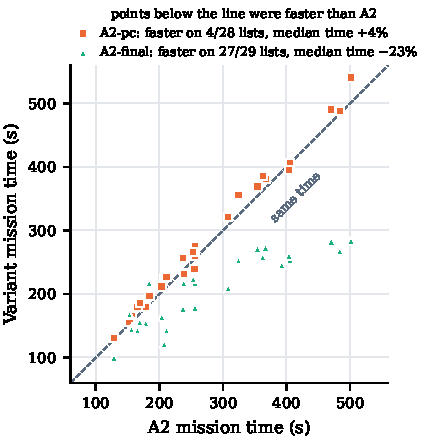
\includegraphics[width=\columnwidth]{fig7_phase2_paired}
\caption{List-by-list mission time of each variant against the original stack, for lists both completed. Points below the diagonal were faster than A2.}
\label{fig:p2pair}
\end{figure}

C2 had shown exact ordering completing only 15 of 30 lists under the default check. C2 used different lists, so the rates compare, not individual lists. Together, the results show that the two changes are complementary: the relaxed check alone mainly removes recoveries, ordering alone saves time but loses missions, and only the combination gives both.

\subsection{Hardware-in-the-Loop Bench Test}
\label{sec:hil}
The stack's velocity commands were connected to the cart's drive hardware on a bench (Fig.~\ref{fig:bench}): two DC motors with Hall encoders on SmartElex 15S drivers, commanded by an Arduino Uno at up to $\pm60$ of 255 PWM, with a 300~ms command watchdog and a hardware E-stop input. Person detection (YOLOv8n with ByteTrack) ran on a Raspberry Pi~5 with a USB webcam and sent the person-state flags to the behaviour tree on the laptop over UDP; both were on a phone hotspot, and the Pi was operated over SSH from that laptop. The rest of the stack ran in simulation. Fig.~\ref{fig:hil} shows a 15-minute session logged by the motor bridge at one sample per encoder report (1~s). The behaviour tree spent 240~s in LEAD, 29~s in FOLLOW and 616~s in WAIT, with nine starts and seven stops while moving. The relay logged every change of the person-state flags received from the Pi, and the behaviour tree (10~Hz) logged every mode change. Over 22 flag changes, the tree changed mode a median of 0.12~s after the relay (maximum 0.20~s), except for the first five, within 40~s of the Pi's data starting, which took 0.6--1.0~s. Every change appeared as the matching mode in the motor log within 1.6~s. Nine times the Pi cleared both flags; each time the PWM sent was zero in the first WAIT sample, and in the following 1~s window the right encoder counted at most one pulse (eight pulses once, when stopping from 0.15~m/s). Once the Pi went silent for 1.5~s; the relay held the tree in WAIT until data resumed 0.5~s later.

Driving straight at 0.10~m/s, the right wheel's measured speed was 104~mm/s (median; range 97--105~mm/s, 29 samples). At the follower's 0.15~m/s the right wheel was at the PWM limit and reached about 105~mm/s, so the bench drive cannot yet reach the follower's speed. The left encoder registered one pulse in the whole session while its wheel was commanded, so the left wheel ran without speed feedback. The same encoder had counted 63--101 pulses per second at PWM 40--55 in a calibration run 106~minutes earlier, falling to 26 at PWM 60, which points to an intermittent connection rather than a failed sensor. During a 22~s burst of repeated enrol and lead-me commands from the button window, the tree switched to LEAD for 0.1~s seven times; one of these pulses sent a turn command of $-0.5$~rad/s to the motors, which the 1~s motor log recorded under WAIT. The serial link acknowledged 17\,660 commands and delivered 881 encoder reports without an error. In a bench check before the session, both wheels counted no pulses from 1.6~s after commands stopped, with the Uno's 300~ms watchdog as the only stop.

Two shopping lists, of one and five items, ran in the simulated store during the session, and the goal-reached race of Section~\ref{sec:disc} was observed directly. After each arrival the planner re-planned to the reached goal every 2~s, and the hand-over published ``goal reached'' each time. Two of the four goals the shopping manager published were marked complete within 2~ms of being published and were skipped. The delay from a person leaving the frame to the Pi clearing its flags was not logged, and with 1~s motor samples the flag-to-stop delay is bounded, not measured.

\begin{figure}[t]
\centering
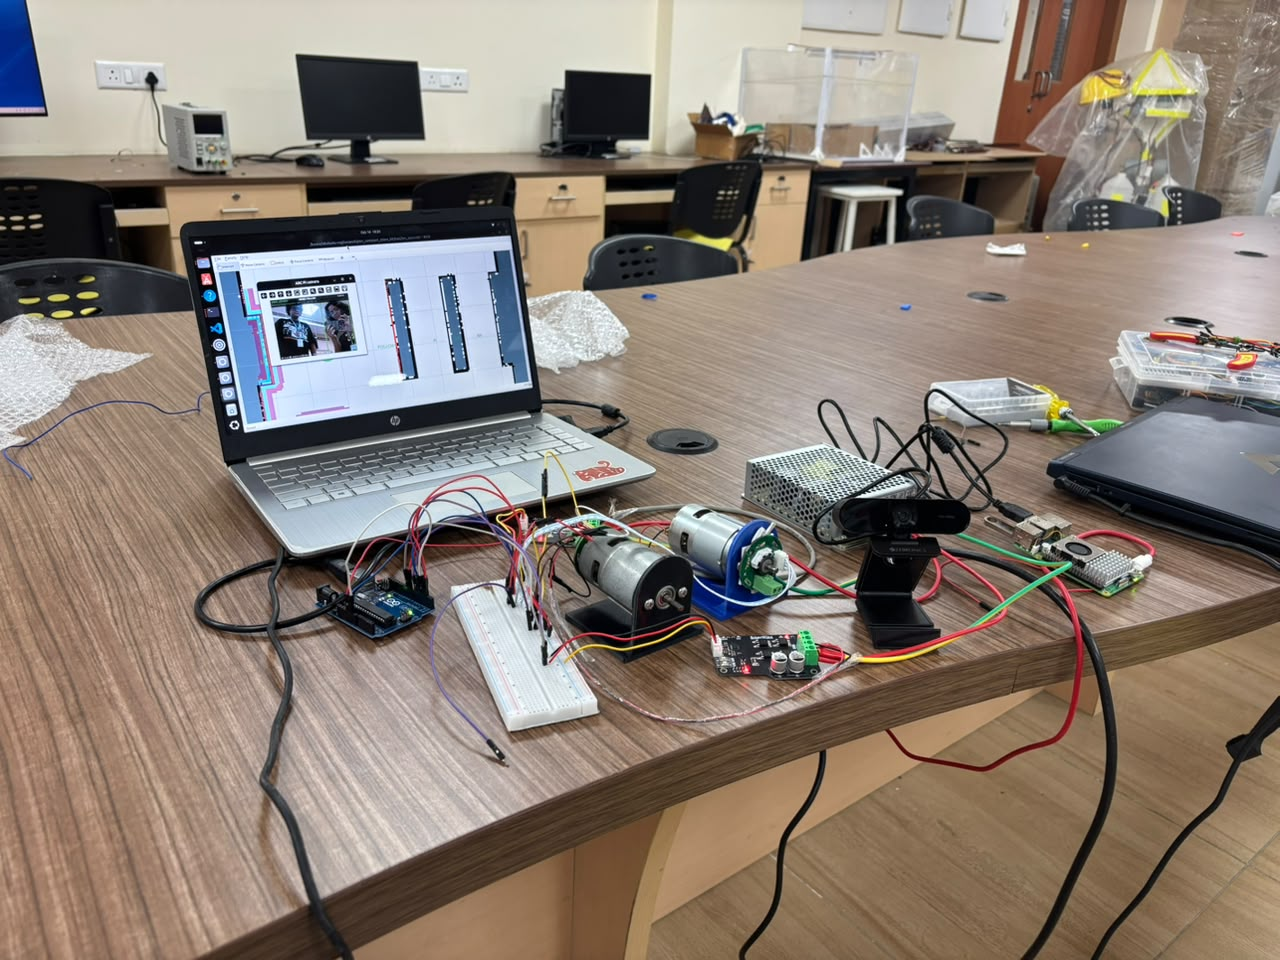
\includegraphics[width=\columnwidth]{fig9_bench.jpg}
\caption{Bench hardware-in-the-loop setup: laptop running the stack, Raspberry Pi~5 with USB webcam, Arduino Uno, two SmartElex drivers and the two encoder drive motors.}
\label{fig:bench}
\end{figure}

\begin{figure}[t]
\centering
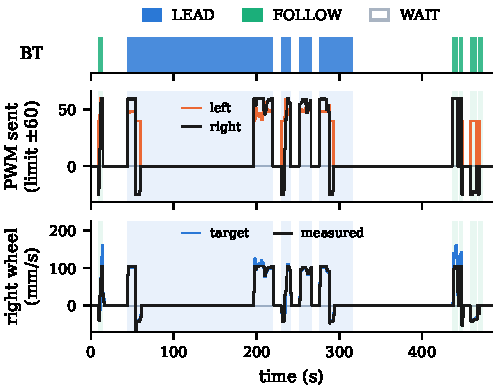
\includegraphics[width=\columnwidth]{fig8_hil_timeline}
\caption{Bench session logged by the motor bridge (1~s samples). Top: behaviour-tree mode. Middle: PWM sent to each driver. Bottom: right-wheel target and encoder-measured speed. The left encoder gave no pulses (Section~\ref{sec:hil}).}
\label{fig:hil}
\end{figure}

\section{Discussion}
\label{sec:disc}
Five integration-level properties matter more for reliability than the choice of algorithm in any one module.
\begin{enumerate}
\item \textit{A default parameter causes most aborts.} Nav2's default progress check, which ARC never overrides, is too strict for an assistive robot at 0.10--0.15~m/s. Relaxing it removed all 62 aborts in A2-pc.
\item \textit{The hand-over has no replanning or recovery.} Unmapped obstacles are left to the local controller alone, and an abort becomes a stall.
\item \textit{A goal-reached race between planner and mission manager.} After an arrival, the planner may replan to the previous goal, and the hand-over can report that path as reached immediately. In C2 the kit's guard caught a ``goal reached'' message while the robot was more than 1~m from its current goal 96 times in 543 legs. This race is the likely cause; in the bench session it was traced event by event and skipped two of four goals (Section~\ref{sec:hil}). ARC's shopping manager, which advances on the first ``goal reached'', is exposed to it.
\item \textit{Lidar odometry has no recovery from a failed match.} After obstacle contact the failure was permanent. An automatic odometry reset is a candidate remedy, not yet tested.
\item \textit{Lidar odometry protects re-localisation.} With wheel odometry, RTAB-Map rejected matches that disagreed with the drifted odometry and stopped correcting.
\end{enumerate}
Path-cost ordering clearly saves time, but its benefit is realised only once the progress check stops short legs from aborting (Section~\ref{sec:p2}).

\textit{Recommendation (phase~3).} Adopt both changes together. First, set the controller's progress check explicitly to 0.25~m within 20~s instead of relying on the Nav2 default. Second, order the shopping list by path cost with the exact solver, which takes under 5~ms for 12 items. Together they completed every A2 list in a quarter less time. Two cautions apply. A lenient progress check prolongs pushing when the robot is pressed against an obstacle, so it should be paired with contact or slip detection on the cart (safety requirements for personal care robots are set out in ISO~13482 \cite{iso13482}); the single shelf contact in A2-pc is the evidence for this, not a measured rate. And ordering raises turning per metre, which matters for passenger comfort on a cart. The hand-over's lack of replanning, the goal-reached race and the missing odometry recovery are not addressed by these two changes and remain the next targets. A second ordering option, ending every route at the checkout counter, has been implemented and is evaluated separately.

\section{Limitations}
All results come from simulation with a stand-in robot that is smaller and lighter than the cart, in one store layout with static shelves and no people, so human-aware navigation \cite{kruse2013,moller2021} was not evaluated. A4 used static boxes only. The cart prototype currently has drive motors, Hall-sensor wheel encoders and a webcam but no lidar, so the localisation and obstacle results do not transfer to it as built. An offline footprint check on the same map, for a standard 180~L trolley ($1000\times610$~mm), bounds how far the store geometry transfers. With a 0.355~m radius (half the width plus 0.05~m, for driving straight), all 9 stops remained reachable with no goal moved, and routes were 9.7\% longer than on the test grid. With a 0.586~m radius (half the diagonal, for turning on the spot), all 9 stops were reachable only with goals moved up to 0.85~m away from the shelf. A full-size cart can therefore use the aisles, but cannot turn on the spot at every stop. Both radii are circular bounds on a rectangular footprint. Navigation ran on a laptop. Perception ran on a Raspberry Pi~5 in the bench test, but its frame rate was not logged, so no claim is made about Raspberry Pi performance. The bench test drove unloaded motors, not the cart. With 20--30 trials per configuration, only large effects are detectable; rare events such as the single A2-pc contact cannot be given a rate. Maps were rebuilt for each session, and session boundaries are recorded. A2-pc ran in three sessions: lists 0--4, then 6--29 after a localisation loss, then list 5, which a 0-based resume index had skipped. For the later sessions the mapping drive's in-run drift limit was relaxed from 0.15~m to 0.30~m after two drives were stopped at 0.16~m and 0.26~m; the acceptance checks on the finished map were unchanged. The kit's goal re-send is not part of ARC, so recoveries are reported separately. Contact is computed geometrically, not sensed.

\section{Conclusion and Future Work}
ARC's navigation stack localises to within a few centimetres and completes nearly all shopping missions in simulation, but only with external re-sends. Its weaknesses are integration-level and traceable to code: a default progress check, a hand-over without replanning or recovery, a goal-reached race, and lidar-odometry failure after contact. Path-cost ordering cuts driving time by a quarter to two-fifths. In phase~2, relaxing the progress check removed the aborts but not the failures, and slowed missions slightly; combined with exact ordering, it completed all 30 lists in 26\% less time and 38\% less distance than the original stack. We therefore recommend adopting both together, with contact detection on the cart. On a bench, the real motors followed the stack's commands under webcam person detection and stopped within one telemetry period of each switch to WAIT. Next steps are restoring left-wheel speed feedback, logging the camera-to-stop delay and the Raspberry Pi frame rate, and integrating a 2D lidar on the cart.

\section*{Acknowledgment}
The authors thank the School of Mechanical Engineering, Vellore Institute of Technology, Chennai, for laboratory facilities and academic support during Capstone Project~1 (BMHA497J). The evaluation relied on open-source software from the ROS~2, Nav2, RTAB-Map, Gazebo and Ultralytics communities. An AI assistant (Claude, Anthropic) was used to help write the test kit, analyse the logs and draft the text; all results come from the authors' logged experiments, and the authors take full responsibility for the content.

\begin{thebibliography}{99}
% In order of first citation.
\bibitem{estember2017}
R.~D. Estember and M.~H.~P. Berdan, ``Ergonomic assessment and design improvement of shopping carts for the satisfaction of buyers in grocery stores and supermarkets,'' in \emph{Proc. IEEE Int. Conf. Ind. Eng. Eng. Manage. (IEEM)}, 2017.

\bibitem{yueh2026}
H.-P. Yueh, W.~Lin, C.-H. Chen, F.-H. Chang, and L.-C. Fu, ``From automation to cognition: A contextual design approach for enhancing elderly patron services with proactive and memory-aware library robots,'' \emph{The Electronic Library}, vol.~44, no.~1, pp.~204--226, 2026.

\bibitem{kulyukin2005}
V.~Kulyukin, C.~Gharpure, and J.~Nicholson, ``RoboCart: Toward robot-assisted navigation of grocery stores by the visually impaired,'' in \emph{Proc. IEEE/RSJ Int. Conf. Intell. Robots Syst. (IROS)}, 2005.

\bibitem{su2016}
H.~Su, Y.~Zhang, J.~Li, and J.~Hu, ``The shopping assistant robot design based on ROS and deep learning,'' in \emph{Proc. 2nd Int. Conf. Cloud Comput. Internet Things (CCIOT)}, Dalian, China, 2016, pp.~173--176, doi:10.1109/CCIOT.2016.7868328.

\bibitem{chiang2016}
H.-H. Chiang, W.-T. You, S.-H. Lin, W.-C. Shih, Y.-T. Liao, J.-S. Lee, and Y.-L. Chen, ``Development of smart shopping carts with customer-oriented service,'' in \emph{Proc. Int. Conf. Syst. Sci. Eng. (ICSSE)}, 2016.

\bibitem{sales2016}
J.~Sales, J.~V. Mart\'i, R.~Mar\'in, E.~Cervera, and P.~J. Sanz, ``CompaRob: The shopping cart assistance robot,'' \emph{Int. J. Distrib. Sensor Netw.}, vol.~12, no.~2, art.~4781280, 2016, doi:10.1155/2016/4781280.

\bibitem{yao2026}
H.~Yao, J.~Peng, H.~Dai, F.~Li, and T.~C. Lueth, ``A shopping service robot framework with visual-WEM tracking and intersection-aware following,'' \emph{IEEE Robot. Autom. Lett.}, vol.~11, no.~4, pp.~4889--4896, 2026, doi:10.1109/LRA.2026.3668142.

\bibitem{nishimura2007}
S.~Nishimura, H.~Takemura, and H.~Mizoguchi, ``Development of attachable modules for robotizing daily items---Person following shopping cart robot,'' in \emph{Proc. IEEE Int. Conf. Robot. Biomimetics (ROBIO)}, 2007, pp.~1506--1511, doi:10.1109/ROBIO.2007.4522387.

\bibitem{kohtsuka2011}
T.~Kohtsuka, T.~Onozato, H.~Tamura, S.~Katayama, and Y.~Kambayashi, ``Design of a control system for robot shopping carts,'' in \emph{Knowledge-Based Intell. Inf. Eng. Syst. (KES 2011)}, LNCS vol.~6881, 2011, pp.~280--288, doi:10.1007/978-3-642-23851-2\_29.

\bibitem{ramaraj2024}
V.~Ramaraj, A.~Paralikar, E.~J. Lee, S.~M. Anwar, and R.~Monfaredi, ``Development of a modular real-time shared-control system for a smart wheelchair,'' \emph{J. Signal Process. Syst.}, vol.~96, no.~3, pp.~203--214, 2024, doi:10.1007/s11265-022-01828-6.

\bibitem{kang2026}
D.~Kang, E.~Kang, J.~Park, and S.-D. Eun, ``Universal bidirectional wheelchair propulsion system: Design and development of a detachable mechanism for manual wheelchair users with spinal cord injury,'' \emph{Appl. Sci.}, vol.~16, art.~2505, 2026, doi:10.3390/app16052505.

\bibitem{satake2009}
J.~Satake and J.~Miura, ``Robust stereo-based person detection and tracking for a person following robot,'' in \emph{Proc. IEEE ICRA Workshop People Detection Tracking}, Kobe, Japan, 2009.

\bibitem{luber2011}
M.~Luber, L.~Spinello, and K.~O. Arras, ``People tracking in RGB-D data with on-line boosted target models,'' in \emph{Proc. IEEE/RSJ Int. Conf. Intell. Robots Syst. (IROS)}, 2011.

\bibitem{basso2012}
F.~Basso, M.~Munaro, S.~Michieletto, E.~Pagello, and E.~Menegatti, ``Fast and robust multi-people tracking from RGB-D data for a mobile robot,'' in \emph{Proc. Int. Conf. Social Robotics (ICSR)}, Springer, 2012.

\bibitem{aye2019}
Y.~Y. Aye, K.~Thiha, M.~M.~M. Pyu, and K.~Watanabe, ``A deep neural network based human following robot with fuzzy control,'' in \emph{Proc. IEEE Int. Conf. Robot. Biomimetics (ROBIO)}, Dali, China, 2019, pp.~720--725.

\bibitem{yong2022}
C.~L. Yong, B.~H. Kwan, D.~W.~K. Ng, and H.~S. Sim, ``Human tracking and following using machine vision on a mobile service robot,'' in \emph{Proc. IEEE 10th Conf. Syst. Process Control (ICSPC)}, Melaka, Malaysia, 2022, pp.~274--279, doi:10.1109/ICSPC55597.2022.10001803.

\bibitem{yaseen2024}
M.~Yaseen, ``What is YOLOv8: An in-depth exploration of the internal features of the next-generation object detector,'' arXiv:2408.15857, 2024.

\bibitem{zhang2022}
Y.~Zhang, P.~Sun, Y.~Jiang, D.~Yu, F.~Weng, Z.~Yuan, P.~Luo, W.~Liu, and X.~Wang, ``ByteTrack: Multi-object tracking by associating every detection box,'' in \emph{Proc. Eur. Conf. Comput. Vis. (ECCV)}, 2022.

\bibitem{ratliff1983}
H.~D. Ratliff and A.~S. Rosenthal, ``Order-picking in a rectangular warehouse: A solvable case of the traveling salesman problem,'' \emph{Oper. Res.}, vol.~31, no.~3, pp.~507--521, 1983, doi:10.1287/opre.31.3.507.

\bibitem{dekoster2007}
R.~de~Koster, T.~Le-Duc, and K.~J. Roodbergen, ``Design and control of warehouse order picking: A literature review,'' \emph{Eur. J. Oper. Res.}, vol.~182, no.~2, pp.~481--501, 2007.

\bibitem{rosenkrantz1977}
D.~J. Rosenkrantz, R.~E. Stearns, and P.~M. Lewis, ``An analysis of several heuristics for the traveling salesman problem,'' \emph{SIAM J. Comput.}, vol.~6, no.~3, pp.~563--581, 1977, doi:10.1137/0206041.

\bibitem{croes1958}
G.~A. Croes, ``A method for solving traveling-salesman problems,'' \emph{Oper. Res.}, vol.~6, no.~6, pp.~791--812, 1958.

\bibitem{held1962}
M.~Held and R.~M. Karp, ``A dynamic programming approach to sequencing problems,'' \emph{J. Soc. Ind. Appl. Math.}, vol.~10, no.~1, pp.~196--210, 1962.

\bibitem{choi2025}
D.~Choi, J.~R. Venepally, and D.~Kim, ``Path-planning and navigation for robots considering human--robot--environment interactions in supermarket environments,'' \emph{Electronics}, vol.~14, no.~11, art.~2111, 2025, doi:10.3390/electronics14112111.

\bibitem{dijkstra1959}
E.~W. Dijkstra, ``A note on two problems in connexion with graphs,'' \emph{Numerische Mathematik}, vol.~1, pp.~269--271, 1959.

\bibitem{macenski2020}
S.~Macenski, F.~Mart\'in, R.~White, and J.~Gin\'es~Clavero, ``The Marathon 2: A navigation system,'' in \emph{Proc. IEEE/RSJ Int. Conf. Intell. Robots Syst. (IROS)}, 2020, pp.~2718--2725.

\bibitem{rosmann2012}
C.~R\"osmann, W.~Feiten, T.~W\"osch, F.~Hoffmann, and T.~Bertram, ``Trajectory modification considering dynamic constraints of autonomous robots,'' in \emph{Proc. 7th German Conf. Robotics (ROBOTIK)}, 2012.

\bibitem{rosmann2017}
C.~R\"osmann, F.~Hoffmann, and T.~Bertram, ``Integrated online trajectory planning and optimization in distinctive topologies,'' \emph{Robot. Auton. Syst.}, vol.~88, pp.~142--153, 2017.

\bibitem{fox1997}
D.~Fox, W.~Burgard, and S.~Thrun, ``The dynamic window approach to collision avoidance,'' \emph{IEEE Robot. Autom. Mag.}, vol.~4, no.~1, pp.~23--33, 1997.

\bibitem{rachman2025}
F.~I. Rachman, ``Improved dynamic window approach using Sugeno fuzzy logic for mobile robot collision avoidance,'' in \emph{Proc. IEEE CENIM}, 2025, doi:10.1109/CENIM67940.2025.11325845.

\bibitem{wu2021}
J.~Wu, X.~Ma, T.~Peng, and H.~Wang, ``An improved timed elastic band (TEB) algorithm of autonomous ground vehicle (AGV) in complex environment,'' \emph{Sensors}, vol.~21, no.~24, art.~8312, 2021.

\bibitem{li2025}
B.~Li, K.~Ni, F.~Zhou, Y.~Li, W.~Huang, H.~Jiang, and F.~Liu, ``Research on robot path planning based on fused Dijkstra and TEB algorithms,'' \emph{J. Mech. Sci. Technol.}, vol.~39, no.~8, pp.~4651--4660, 2025, doi:10.1007/s12206-025-0738-8.

\bibitem{murartal2017}
R.~Mur-Artal and J.~D. Tard\'os, ``ORB-SLAM2: An open-source SLAM system for monocular, stereo, and RGB-D cameras,'' \emph{IEEE Trans. Robot.}, vol.~33, no.~5, pp.~1255--1262, 2017.

\bibitem{tourani2022}
A.~Tourani, H.~Bavle, J.~L. Sanchez-Lopez, and H.~Voos, ``Visual SLAM: What are the current trends and what to expect?,'' \emph{Sensors}, vol.~22, no.~23, art.~9297, 2022.

\bibitem{shan2020}
T.~Shan, B.~Englot, D.~Meyers, W.~Wang, C.~Ratti, and D.~Rus, ``LIO-SAM: Tightly-coupled lidar inertial odometry via smoothing and mapping,'' in \emph{Proc. IEEE/RSJ Int. Conf. Intell. Robots Syst. (IROS)}, 2020, pp.~5135--5142.

\bibitem{altawil2025}
B.~Al-Tawil, A.~Candemir, M.~Jung, and A.~Al-Hamadi, ``Mobile robot navigation with enhanced 2D mapping and multi-sensor fusion,'' \emph{Sensors}, vol.~25, no.~8, art.~2408, 2025.

\bibitem{pomerleau2013}
F.~Pomerleau, F.~Colas, R.~Siegwart, and S.~Magnenat, ``Comparing ICP variants on real-world data sets,'' \emph{Auton. Robots}, vol.~34, no.~3, pp.~133--148, 2013.

\bibitem{labbe2019}
M.~Labb\'e and F.~Michaud, ``RTAB-Map as an open-source lidar and visual simultaneous localization and mapping library for large-scale and long-term online operation,'' \emph{J. Field Robot.}, vol.~36, no.~2, pp.~416--446, 2019, doi:10.1002/rob.21831.

\bibitem{colledanchise2018}
M.~Colledanchise and P.~\"Ogren, \emph{Behavior Trees in Robotics and AI: An Introduction}. Boca Raton, FL, USA: CRC Press, 2018.

\bibitem{iovino2022}
M.~Iovino, E.~Scukins, J.~Styrud, P.~\"Ogren, and C.~Smith, ``A survey of behavior trees in robotics and AI,'' \emph{Robot. Auton. Syst.}, vol.~154, art.~104096, 2022.

\bibitem{ogren2022}
P.~\"Ogren and C.~I. Sprague, ``Behavior trees in robot control systems,'' \emph{Annu. Rev. Control Robot. Auton. Syst.}, vol.~5, pp.~81--107, 2022.

\bibitem{macenski2022}
S.~Macenski, T.~Foote, B.~Gerkey, C.~Lalancette, and W.~Woodall, ``Robot Operating System 2: Design, architecture, and uses in the wild,'' \emph{Sci. Robot.}, vol.~7, no.~66, art.~eabm6074, 2022.

\bibitem{koenig2004}
N.~Koenig and A.~Howard, ``Design and use paradigms for Gazebo, an open-source multi-robot simulator,'' in \emph{Proc. IEEE/RSJ Int. Conf. Intell. Robots Syst. (IROS)}, 2004, pp.~2149--2154.

\bibitem{macenski2023}
S.~Macenski, S.~Singh, F.~Mart\'in, and J.~Gin\'es, ``Regulated pure pursuit for robot path tracking,'' \emph{Auton. Robots}, vol.~47, pp.~685--694, 2023.

\bibitem{wilcoxon1945}
F.~Wilcoxon, ``Individual comparisons by ranking methods,'' \emph{Biometrics Bull.}, vol.~1, no.~6, pp.~80--83, 1945.

\bibitem{thrun2005}
S.~Thrun, W.~Burgard, and D.~Fox, \emph{Probabilistic Robotics}. Cambridge, MA, USA: MIT Press, 2005.

\bibitem{iso13482}
\emph{Robots and Robotic Devices---Safety Requirements for Personal Care Robots}, ISO~13482:2014, International Organization for Standardization, 2014.

\bibitem{kruse2013}
T.~Kruse, A.~K. Pandey, R.~Alami, and A.~Kirsch, ``Human-aware robot navigation: A survey,'' \emph{Robot. Auton. Syst.}, vol.~61, no.~12, pp.~1726--1743, 2013.

\bibitem{moller2021}
R.~M\"oller, A.~Furnari, S.~Battiato, A.~H\"arm\"a, and G.~M. Farinella, ``A survey on human-aware robot navigation,'' \emph{Robot. Auton. Syst.}, vol.~145, art.~103837, 2021.
\end{thebibliography}

\end{document}
